\documentclass[12pt,txfonts]{paper}
\usepackage{verbatim,rotating,url}
\usepackage{pstricks}
\usepackage[numbers,sort&compress]{natbib}

%%% Bold symbols

\DeclareSymbolFont{mathbold}{OML}{cmm}{b}{it}
\DeclareMathSymbol{\bA}{\mathord}{mathbold}{`A}
\DeclareMathSymbol{\bP}{\mathord}{mathbold}{`P}
\DeclareMathSymbol{\br}{\mathord}{mathbold}{`r}

\renewcommand{\baselinestretch}{1.05}
\raggedbottom
\parindent 0pt
\parskip 6pt
\newenvironment{newverbatim}%
{\renewcommand{\baselinestretch}{1.0}\verbatim}%
{\endverbatim}
\newenvironment{example}%
{\begin{list}{\setlength\topsep{0pt}\setlength\leftmargin{2em}%
\setlength\parskip{0pt}\setlength\partopsep{0pt}}{%
\item[]\ignorespaces}}
{\unskip\end{list}}
\bibliographystyle{cpl}
% \setcitestyle{numbers}
% \citestyle{cpl}
\let\cite=\citep
\frenchspacing

\let\ring=\r
\newcommand{\angstrom}{\unskip\ensuremath{\,\hbox{\ring A}}}
\newcommand\kJpermol{\ensuremath{\,{\rm kJ\,mol}^{-1}}}

\graphicspath{{./pictures/}}
\renewcommand\textfraction{0.1}
\renewcommand\topfraction{0.8}
\renewcommand\floatpagefraction{0.6}

\begin{document}


\begin{center}
\textbf{Distributed Multipole Analysis of Gaussian wavefunctions\\[3pt]
GDMA version 2.3.0\\[4 pt]
Anthony J. Stone}
\end{center}

\section{Introduction}

The GDMA program carries out Distributed Multipole Analysis of
wavefunctions expressed in terms of Gaussian atomic orbitals.
The calculation can be carried out directly in the CamCASP
program\cite{CamCASP5.9}, or
by using as input the formatted checkpoint (``.fchk'') file
that can be generated using the Psi4 quantum chemistry code\cite{psi4} or the
Gaussian system of programs\cite{Gaussian16}
.
If you find any bugs, please send email to Anthony
Stone, ajs1@cam.ac.uk. Comments and corrections would also be welcome.
Instructions given here refer to the use of the program with a .fchk file.
Most of the information also applies to the {\sc CamCASP} package; for
the differences, see the {\sc CamCASP} documentation. CamCASP does not
as yet provide for basis sets that include $h$ basis functions.

The recommended procedure for using the program is to
construct a small data file of the following form:\\
\hspace*{2 em}\verb/FILE/ \emph{checkpointfile} %
\verb/[DENSITY/ \emph{density-type}\verb/]/\\
\hspace*{2 em}\verb/[NAMES/\\
\hspace*{2 em}\quad\emph{List of atom names, on one
 or more lines}\verb/]/\\
\hspace*{2 em}\verb/MULTIPOLES/\\
\hspace*{2 em}\quad\emph{subcommands, described below}\\
\hspace*{2 em}\verb/START/\\
For use with {\sc CamCASP}, the first line is omitted, and the
remaining commands should appear between \verb+BEGIN GDMA+ and 
\verb+END+ lines in the {\sc CamCASP} input file. 
The keywords shown in uppercase may be typed in upper, lower or mixed
case. The \verb/DENSITY/ specification is optional; the
default is to read the SCF density matrix from the checkpoint file.
(Here and later, square brackets denote optional items. The square
brackets themselves are not part of the data.)
Any other density matrix that appears in the checkpoint file may be
specified; if the name contains spaces it must be enclosed in single
or double quotes. The \verb/NAMES/
command is optional, but may be needed for some DMA options. If it is
provided, the atom names should be listed, separated by spaces, in the
order that the atoms appear in the checkpoint file. (At this point the
program knows how many atoms there are, but the checkpoint file
doesn't include their names.) If the
\verb/NAMES/ command is omitted, each atom is given a name which is
the chemical symbol corresponding to its atomic number. The
\verb/MULTIPOLES/ command may be repeated to obtain DMAs with
different options, for example with different choices of multipole
sites. The \verb/FILE/ command may be repeated to read another
checkpoint file, or a different density from the same file.

Other options that may appear are:

\hspace*{2 em}\verb/VERBOSE/\\
This may precede the \verb+FILE+ command, and causes the program to
print information about the data read from the checkpoint file. It is
primarily for debugging purposes and should not normally be needed.

\hspace*{2 em}\verb/ANGSTROM/\\
If needed, this should follow the \verb+FILE+ command unless the atom
coordinates in 
the formatted checkpoint file are in {\aa}ngstrom instead of atomic units.
Any length values given in subsequent \verb+MULTIPOLES+ sections of the data
(see below) will then be taken to be in {\aa}ngstrom, and coordinates printed
by the program will be given in {\aa}ngstrom also, instead of atomic units.

% \pagebreak
\hspace*{2 em}\verb/BOHR/\\
This can be used to cancel the effect of a previous \verb/ANGSTROM/
command, but will not normally be needed.

\hspace*{2 em}\verb/AU/\\
Multipole moments printed by the program will be in atomic units,
$ea_0^n$ for moments of rank $n$. (See sec.~\ref{multipoles} below for
the definition of rank.) This is the default.

\hspace*{2 em}\verb/SI/\\
\label{SI}%
Multipole moments printed by the program will be in SI units, Cm$^n$
for moments of rank $n$, but multiplied by a factor $10^{20+10n}$. For
example, a dipole moment (rank 1) with a value of $0.7\times10^{-30}$
Cm will be printed as $0.7$.

For information on generating the Gaussian formatted checkpoint file,
see the Gaussian documentation. In brief, you need a line at the
beginning of your Gaussian input of the form\\
\hspace*{2 em}\verb:%chk=:\emph{chkfile}\\
which causes Gaussian to produce a binary checkpoint file called
\emph{chkfile}. There is a Gaussian utility \verb+formchk+ which
converts this into the formatted checkpoint file used by GDMA.

For Psi4, see the Psi4 documentation. In brief, if running under
psithon, use something like\\[6pt]
\hspace{1em}\begin{minipage}[c]{100mm}
\begin{verbatim}
energy, wfn = psi4.energy("PBE0", return\_wfn=True)
psi4.fchk(wfn,"pbe0.fchk")
\end{verbatim}
  \end{minipage}

\section {Distributed Multipole Analysis}

Distributed Multipole Analysis or DMA is a technique for describing a
molecular charge distribution by using
local multipoles at a number of sites within a molecule. It gives a
much more accurate representation of the charge density than a
single-point multipole expansion, even for small molecules. For
details see \S\ref{multipoles} below. Note that the accuracy of the
description depends on the inclusion of site dipoles, quadrupoles and
possibly higher moments. If you need a point-charge model, the charges
from the distributed multipole analysis are not suitable, but see
\S\ref{subsec:ptcharge} for suggestions. The sites
are usually the nuclei, but existing sites can be omitted and
new sites added. The multipoles are the charges,
dipoles, quadrupoles, etc., up to some limit, which can be as high as
rank 10. The limit need not be the same on every atom. For example the
following 
calculation would give multipoles up to rank 4 (hexadecapole) on the
oxygen atom, but only up to rank 1 on the hydrogen atoms. (Higher
moments on hydrogen atoms are usually very small.) In a case like
this, the higher moments on the H atoms are
transferred to the nearest atom with a higher limit, here the oxygen,
and the overall molecular moments are correct up to the highest rank
specified, rank 4 in this case. (See below, pp.~\pageref{p:switch}ff, for
an explanation of the \verb+SWITCH+ and \verb+RADIUS+ commands.)\\
\hspace*{2 em}\verb/MULTIPOLES/\\
\hspace*{2 em}\verb/LIMIT 4/\\
\hspace*{2 em}\verb/LIMIT 1 H/\\
\hspace*{2 em}\verb/SWITCH 4.0/\\
\hspace*{2 em}\verb/RADIUS H 0.35/\\
\hspace*{2 em}\verb/START/\\
When used with the output file from a B3LYP calculation on water,
using the aug-cc-pVTZ basis set, the
output is as shown %in Figure~\ref{fig:H2O}.
below.  On the oxygen one gets the
charge (Q00), the components of the dipole (Q1), the quadrupole (Q2),
octopole (Q3) and hexadecapole (Q4) moments, while on the hydrogen one
gets only the charge and dipole moment. The components are expressed 
in terms of spherical harmonic definitions (see below). Only the
non-zero moments are printed.
% \pagebreak
% \begin{figure}
\small
% \caption{Program output for a calculation on water (see text).}
% \label{fig:H2O}
\renewcommand{\baselinestretch}{1.0}\small
\begin{verbatim}
O          x =  0.000000  y =  0.000000  z =  0.116982
           Maximum rank =  4   Relative radius =  0.650
                   Q00  =  -0.276214
|Q1| =   0.484939  Q10  =  -0.484939
|Q2| =   1.669447  Q20  =   0.126597  Q22c =  -1.664640
|Q3| =   3.360888  Q30  =   1.303370  Q32c =   3.097869
|Q4| =   6.929535  Q40  =  -3.612674  Q42c =  -5.030396  Q44c =   3.108402

H          x =  0.000000  y =  0.763556  z = -0.467927
           Maximum rank =  1   Relative radius =  0.350
                   Q00  =   0.138107
|Q1| =   0.031927  Q10  =   0.031774  Q11s =  -0.003124

H          x = -0.000000  y = -0.763556  z = -0.467927
           Maximum rank =  1   Relative radius =  0.350
                   Q00  =   0.138107
|Q1| =   0.031927  Q10  =   0.031774  Q11s =   0.003124

Total multipoles
referred to origin at x =   0.000000,  y =    0.000000,  z =    0.000000
                   Q00  =  -0.000000
|Q1| =   0.726696  Q10  =  -0.726696
|Q2| =   2.164751  Q20  =  -0.276239  Q22c =  -2.147054
|Q3| =   3.481250  Q30  =   1.811733  Q32c =   2.972663
|Q4| =   5.620281  Q40  =  -2.635421  Q42c =  -3.021910  Q44c =   3.938297
\end{verbatim}
% \end{figure}

\clearpage
\normalsize
\subsection{Definitions of multipole moments}
\label{multipoles}

The spherical
harmonic multipole $Q_{lk}$ is defined as
\begin{equation*}
Q_{lk} = \int R_{lk}({\bf r}) \rho({\bf r}) {\rm d}^3{\bf r}
\end{equation*}
where $\rho({\bf r})$ is the total charge density, and the regular
solid harmonics $R_{lk}({\bf r})$ are given in Table~1. For those who
prefer the cartesian definitions of multipole moments the relationships
between spherical harmonic and cartesian definitions up to
hexadecapole are given in Table~2.
There are fewer components of the multipole moments in the spherical form
than in the cartesian form (except for the charge and dipole) as the
components of the cartesian multipoles are not all independent.

The quantities listed as \verb+|Qn|+ in the program output are the
magnitudes of the multipole moments, defined by
\begin{equation*}
|Q_n| = \Bigl( \sum_k |Q_{nk}|^2 \Bigr)^{1/2}.
\end{equation*}
They are independent of axis system, and $|Q_1|$ coincides with
the usual expression for the magnitude of the dipole moment.

As well as the distributed multipoles, the program prints the total multipoles
referred to the origin of the coordinate frame. Components which are zero
are not printed, except for the total charge.

All moments are usually given in atomic units, $ea_0^k$ for moments of rank
$k$, but it is possible to have them printed in SI units instead
(\verb+SI+ command, p.~\pageref{SI}).

\newcommand{\half}{\tfrac{1}{2}}
\begin{table}
\caption{Regular solid harmonics}
\parbox[t]{120pt}{%
\begin{align*}
R_{00}&=1\\
R_{10}&=z\\
R_{11c}&=x\\
R_{11s}&=y\\
R_{20}&=\half(3z^2-r^2)\\
R_{21c}&= \sqrt 3 xz\\
R_{21s}&= \sqrt 3 yz\\
R_{22c}&= \sqrt {\tfrac{3}{4}} (x^2-y^2)\\
R_{22s}&= \sqrt 3 xy\\
\end{align*}}
\hfill
\parbox[t]{130pt}{%
\begin{align*}
R_{30}&=\half (5z^3-3zr^2)\\
R_{31c}&=\sqrt {\tfrac{3}{8}} x(5z^2-r^2)\\
R_{31s}&=\sqrt {\tfrac{3}{8}} y(5z^2-r^2)\\
R_{32c}&=\sqrt {\tfrac{15}{4}} z(x^2-y^2)\\
R_{32s}&=\sqrt {15} xyz\\
R_{33c}&=\sqrt {\tfrac{5}{8}} (x^3-3xy^2)\\
R_{33s}&=\sqrt {\tfrac{5}{8}} (3x^2y-y^3)
\end{align*}}
\hfill
\parbox[t]{170pt}{%
\begin{align*}
R_{40}&=\tfrac{1}{8} (35z^4-30z^2r^2+3r^4)\\
R_{41c}&=\sqrt {\tfrac{5}{8}} (7xz^3-3xzr^2)\\
R_{41s}&=\sqrt {\tfrac{5}{8}} (7yz^3-3yzr^2)\\
R_{42c}&=\sqrt {\tfrac{5}{16}} (x^2-y^2)(7z^2-r^2)\\
R_{42s}&=\sqrt {\tfrac{5}{4}} xy(7z^2-r^2)\\
R_{43c}&=\sqrt {\tfrac{35}{8}} z(x^3-3xy^2)\\
R_{43s}&=\sqrt {\tfrac{35}{8}} z(3x^2y-y^3)\\
R_{44c}&=\sqrt {\tfrac{35}{64}} (x^4-6x^2y^2+y^4)\\
R_{44s}&=\sqrt {\tfrac{35}{4}} (x^3y-xy^3)
\end{align*}}
\hrule
\end{table}

% \begin{table}
% \caption{Relationship between spherical-tensor and cartesian-tensor
% form of multipole moments}
% \parbox[t]{110pt}{%
% \begin{align*}
% Q_{10}&=\mu_z\\
% Q_{11c}&=\mu_x\\
% Q_{11s}&=\mu_y\\
% Q_{20}&=\Theta_{zz}\\
% Q_{21c}&=\sqrt \casefrac{4}/{3} \Theta_{xz}\\
% Q_{21s}&=\sqrt \casefrac{4}/{3} \Theta_{yz}\\
% Q_{22c}&=\sqrt \casefrac{1}/{3} (\Theta_{xx}-\Theta_{yy})\\
% Q_{22s}&=\sqrt \casefrac{4}/{3} \Theta_{xy}\\
% \end{align*}}
% \hfill
% \parbox[t]{130pt}{%
% \begin{align*}
% Q_{30}&=\Omega_{zzz}\\
% Q_{31c}&=\sqrt \casefrac{3}/{2} \Omega_{xzz}\\
% Q_{31s}&=\sqrt \casefrac{3}/{2} \Omega_{yzz}\\
% Q_{32c}&=\sqrt \casefrac{3}/{5} (\Omega_{xxz}-\Omega_{yyz})\\
% Q_{32s}&=\sqrt \casefrac{3}/{5}  2\Omega_{xyz}\\
% Q_{33c}&=\sqrt \casefrac{1}/{10}(\Omega_{xxx}-3\Omega_{xyy})\\
% Q_{33s}&=\sqrt \casefrac{1}/{10} (3\Omega_{xxy}-\Omega_{yyy})\\
% \end{align*}}
% \hfill
% \parbox[t]{180pt}{%
% \begin{align*}
% Q_{40}&=\Phi_{zzzz}\\
% Q_{41c}&=\sqrt \casefrac{8}/{5} \Phi_{xzzz}\\
% Q_{41s}&=\sqrt \casefrac{8}/{5} \Phi_{yzzz}\\
% Q_{42c}&=\sqrt \casefrac{4}/{5} (\Phi_{xxzz}-\Phi_{yyzz})\\
% Q_{42s}&=\sqrt \casefrac{16}/{5} \Phi_{xyzz}\\
% Q_{43c}&=\sqrt \casefrac{8}/{35} (\Phi_{xxxz}-3\Phi_{xyyz})\\
% Q_{43s}&=\sqrt \casefrac{8}/{35} (3\Phi_{xxyz}-\Phi_{yyyz})\\
% Q_{44c}&=\sqrt \casefrac{1}/{35} (\Phi_{xxxx}-6\Phi_{xxyy}+\Phi_{yyyy})\\
% Q_{44s}&=\sqrt \casefrac{16}/{35} (\Phi_{xxxy}-\Phi{xyyy})
% \end{align*}}
% \hrule
% \end{table}

\begin{sidewaystable}
\begin{center}
\caption{Relationship between spherical-tensor and cartesian-tensor
form of multipole moments}
\parbox[t]{130pt}{%
\begin{align*}
%\begin{minipage}[t]{45mm}
%\openup 1 \jot\halign{\hfill$#$&${}=#$\hfill\cr
\mu_z&=Q_{10}\\
\mu_x&=Q_{11c}\\
\mu_y&=Q_{11s}\\[10pt]
\Theta_{xx} &= -\half Q_{20} + \half \sqrt3 Q_{22c}\\
\Theta_{yy} &= -\half Q_{20} - \half \sqrt3 Q_{22c}\\
\Theta_{zz} &= Q_{20}\\
\Theta_{xy} &= \half\sqrt3 Q_{22s}\\
\Theta_{xz} &= \half\sqrt3 Q_{21c}\\
\Theta_{yz} &= \half\sqrt3 Q_{21s}
\end{align*}}
\qquad
\parbox[t]{140pt}{%
\begin{align*}
%\noalign{\medskip}
\Omega_{xxx} &= \sqrt{\tfrac{5}{8}} Q_{33c}-\sqrt{\tfrac{3}{8}} Q_{31c}\\
\Omega_{xxy} &= \sqrt{\tfrac{5}{8}} Q_{33s}-\sqrt{\tfrac{1}{24}} Q_{31s}\\
\Omega_{xyy} &= -\sqrt{\tfrac{5}{8}} Q_{33c}-\sqrt{\tfrac{1}{24}} Q_{31c}\\
\Omega_{yyy} &= -\sqrt{\tfrac{5}{8}} Q_{33s}-\sqrt{\tfrac{3}{8}} Q_{31s}\\
\Omega_{xxz} &= \sqrt{\tfrac{5}{12}} Q_{32c}-\half Q_{30}\\
\Omega_{xyz} &= \sqrt{\tfrac{5}{12}} Q_{32s}\\
\Omega_{yyz} &= -\sqrt{\tfrac{5}{12}} Q_{32c}-\half Q_{30}\\
\Omega_{xzz} &= \sqrt{\tfrac{2}{3}} Q_{31c}\\
\Omega_{yzz} &= \sqrt{\tfrac{2}{3}} Q_{31s}\\
\Omega_{zzz} &= Q_{30}
\end{align*}}
\qquad
\parbox[t]{190pt}{%
\begin{align*}
%\end{minipage}\qquad\qquad
%\begin{minipage}[t]{60mm}
%\openup 2 \jot\halign{\hfill$#$&${}=#$\hfill\cr
\Phi_{xxxx} &= {\tfrac{3}{8}} Q_{40} -{\tfrac{1}{4}}\sqrt5 Q_{42c}
          + {\tfrac{1}{8}}\sqrt{35}Q_{44c}\\
\Phi_{xxxy} &= {\tfrac{1}{8}}(-\sqrt{5}Q_{42s}+\sqrt{35}Q_{44s})\\
\Phi_{xxyy} &= {\tfrac{1}{8}} Q_{40} - {\tfrac{1}{8}}\sqrt{35}Q_{44c}\\
\Phi_{xyyy} &= -{\tfrac{1}{8}}(\sqrt{5}Q_{42s}+\sqrt{35}Q_{44s})\\
\Phi_{yyyy} &= {\tfrac{3}{8}} Q_{40} + {\tfrac{1}{4}}\sqrt5 Q_{42c}
          + {\tfrac{1}{8}}\sqrt{35}Q_{44c}\\
\Phi_{xxxz} &= {\tfrac{1}{16}}(-3\sqrt{10}Q_{41c}+\sqrt{70}Q_{43c})\\
\Phi_{xxyz} &= {\tfrac{1}{16}}(-\sqrt{10}Q_{41s}+\sqrt{70}Q_{43s})\\
\Phi_{xyyz} &= -{\tfrac{1}{16}}(\sqrt{10}Q_{41c}+\sqrt{70}Q_{43c})\\
\Phi_{yyyz} &= -{\tfrac{1}{16}}(3\sqrt{10}Q_{41s}+\sqrt{70}Q_{43s})\\
\Phi_{xxzz} &= -{\tfrac{1}{2}} Q_{40} + {\tfrac{1}{4}}\sqrt5 Q_{42c}\\
\Phi_{xyzz} &= {\tfrac{1}{4}}\sqrt5 Q_{42s}\\
\Phi_{yyzz} &= -{\tfrac{1}{2}} Q_{40} - {\tfrac{1}{4}}\sqrt5 Q_{42c}\\
\Phi_{xzzz} &= \sqrt{{\tfrac{5}{8}}}Q_{41c}\\
\Phi_{yzzz} &= \sqrt{{\tfrac{5}{8}}}Q_{41s}\\
\Phi_{zzzz} &= Q_{40}
\end{align*}}
%\end{minipage}
%\hrule
\end{center}
\end{sidewaystable}

\subsection {Multipole allocation algorithms}

The original distributed multipole analysis, as set out in the
bibliography\cite{Stone81a,StoneA85,timf}, starts from the expansion
of the electron density in terms of the primitive gaussian basis
functions $\chi_i(\br)$:
\begin{equation}
\chi_i(\br) = N_i x_i^{a_i}y_i^{b_i}z_i^{c_i}\exp[-\zeta_i(\br_i)^2],
\end{equation}
where $\br_i=\br-\bA_i$ is the electron position relative to the
position $\bA_i$ of the primitive Gaussian, $\zeta_i$ is the exponent
and $N_i$ is a normalising factor.
The electron density is then
\begin{equation}
\rho(\br) = \sum_{ij} D_{ij} \chi_i(\br)\chi_j(\br).
\end{equation}
Boys\cite{Boys50} showed that a product of gaussians
$\chi_i(\br)\chi_j(\br)$ can be expressed as a gaussian function
centred at $\bP_{ij}=(\zeta_i\bA_i+\zeta_j\bA_j)/(\zeta_i+\zeta_j)$. The
multipole moments of the associated charge distribution can be
calculated exactly, and in standard DMA they are represented by a
multipole expansion about the nearest site. This procedure is very
fast and efficient, and gives an excellent representation of the
molecular charge distribution.

If the basis set includes very diffuse functions, however, overlap
densities involving them extend over many atoms. In carbon dioxide,
for instance, the product of a diffuse $s$ function on one O atom and
a diffuse $p_z$ function with slightly larger exponent on the C atom
would be formally centred between the C and O, but slightly nearer to
the C atom, and would give rise to charge and dipole contributions
which would be allocated to the C atom. However, much of the electron
density would in fact be in the region of the O atom, and it would
extend to some extent over all three atoms. It would be more
satisfactory to apportion the charge density between the atoms in some
way.

Methods for doing this have been developed in recent years for
handling the integrals of density functional theory. Version 2 of the
GDMA program\cite{Stone05b} uses these methods to calculate the multipole
contributions arising from the overlap of diffuse primitive functions.
Such an approach is not needed for compact basis functions (those with
large $\zeta$) because the overlap densities involving such functions
are well localised in space, and their allocation to the nearest
multipole site is entirely satisfactory. Moreover the grid-based
quadrature used for the diffuse functions is less satisfactory for
highly-peaked functions.

Consequently the program can now use both methods. If the sum of
exponents $\zeta_i+\zeta_j$ for a pair of primitive functions $\chi_i$
and $\chi_j$ is less than a switch value $Z$, the grid-based analysis
is used, and otherwise the original DMA method is used. If $Z=0.0$,
the original DMA algorithm is used throughout. However the default
value is $Z=4.0$, and this is recommended for normal use, especially
with basis sets containing very diffuse functions. The parameters for
the grid-based quadrature can also be specified, but the default
values should be satisfactory in most cases.

\subsection {Options for multipole analysis}

The \verb/MULTIPOLES/ command has various subcommands, two of which,
\verb/LIMIT/ and \verb/RADIUS/, were included in the example dataset.
The \verb/LIMIT/ command sets the maximum rank 
for the DMA analysis. For example, \verb/LIMIT 4/ instructs the
program to calculate multipoles up to hexadecapole only. The highest rank
which can be calculated for non-linear molecules is 10, i.e.
\verb/LIMIT 10/.
\verb/LIMIT 1/ would calculate only charge and dipole on each site, 
\verb/LIMIT 2/ would include the quadrupole moments, and so on.
It is also possible
to set different limits for different sites. For example\\
\hspace*{2 em}\verb/MULTIPOLES/\\
\hspace*{2 em}\verb/LIMIT 4/\\
\hspace*{2 em}\verb/LIMIT 1 H/\\
\hspace*{2 em}\verb/START/\\
would calculate multipoles up to hexadecapole on all sites except
those called `H', where the expansion would terminate with the dipole
moments. If this dataset is used for water, as in the example, the
effects of the higher 
moments on the H atoms are transferred to the O atom, so that the
overall multipole moments for the whole molecule are correct up to the
highest rank specified. This is usually a sensible procedure for H
atoms, where the higher moments are small. The limit for named atoms
is applied to all atoms with the name given, so if different limits
are wanted for atoms of the same element, the \verb/NAMES/ command
must be used to give them distinctive names. The general form of the
\verb/LIMIT/ command is `\verb/LIMIT /$n$ \emph{name name }\dots' or
`\verb/LIMIT /$n$ \verb/ALL/ \emph{aa}'. The latter form applies the
limit to all sites with names starting with `\emph{aa}'. Site names
are always case-sensitive.

The list of sites can be modified using \verb/ADD/ and \verb/DELETE/.
Extra sites can be included in the analysis by using the \verb/ADD/
command:\\
\hspace*{2 em}\verb/ADD/ \emph{name} $x$ $y$ $z$ \verb/[LIMIT/ $n$\verb/] [RADIUS /$r$\verb/]/\\
where $x$, $y$ and $z$ are the cartesian coordinates of the new site
(in atomic units, unless the \verb+ANGSTROM+ command has been used).
Items in square brackets are optional.
The optional \verb+LIMIT+ $n$ sets the maximum rank for this site; if
it is omitted, the current maximum rank is used.
The \verb+RADIUS+ option, if present, sets the radius (see below). If
it is omitted, a value of $0.65\angstrom$ is used.

\verb/DELETE/ removes all sites with the name specified.
For example,\\
\hspace*{2 em}\verb/MULTIPOLES/\\
\hspace*{2 em}\verb/DELETE H/\\
\hspace*{2 em}\verb/START/\\
would remove from the analysis all sites called `H'. This would 
sometimes be done in large molecules to avoid an over-proliferation
of expansion centres. For example one might want to avoid
using the methyl hydrogen atoms as multipole sites in a large
molecule. To delete the methyl hydrogens in methanol but retain  
the OH hydrogen (a common situation where hydrogen bonding is
involved) it would be necessary to use different names for the methyl
and OH hydrogens, perhaps `H' and `Ho' respectively, and then
\verb/DELETE H/ would have the required effect.

% \pagebreak

If you use \verb/DELETE ALL/ then all sites are removed.
In this case you will need to use \verb/ADD/ to provide at least one
site for the expansion. This provides a way to get a single-site
expansion referred to a site other than the origin of coordinates.
However a simpler way is to use the command\\
\hspace*{2 em}\verb/ORIGIN/ $o_x$ $o_y$ $o_z$\\
to specify the origin for the overall multipole moments.

It should perhaps be emphasized once again that whatever sites are
added or deleted, the overall multipole moments will be correct up to
the maximum rank of any site that remains. However, if too few sites
are used, the resulting multipole expansion of the electrostatic
potential or of the electrostatic interaction between molecules may be
inaccurate. See my book for a fuller discussion\cite{timf}.

\label{p:switch}
The switch between the original DMA algorithm and the new grid-based
quadrature can be controlled by the command\\
\hspace*{2 em}\verb/SWITCH /$Z$\\
The default value is $4.0$. To use the original algorithm, use 
\verb/SWITCH 0.0/, but it is important in this case to check that the
results are sensible.

The \verb/GRID/ command controls parameters for the quadrature grid:\\
\hspace*{2 em}\verb/GRID /\emph{options}\\
The options are\\
\hspace*{2 em}\verb/LEBEDEV /$n$\\
Use Lebedev angular quadrature\cite{LebedevL99} with at least $n$
points for each atom.
Lebedev quadrature is the default, but this command is needed if the
number of points is to be changed from the default of 590. Note that a
high value is needed, especially if high-rank multipoles are required,
because they are quite sensitive to the angular behaviour of the
charge density.\\
\hspace*{2 em}\verb/GAUSS-LEGENDRE /$n$\\
Use Gauss--Legendre quadrature in $\theta$ and equally-spaced
intervals in $\phi$, with the total number of points chosen to be at
least $n$.\\
\hspace*{2 em}\verb/RADIAL /$n$\\
Use $n$ points for the radial quadrature (default 80). This value
needs to be large, especially if high-rank multipoles are required,
because they are strongly influenced by the electron density at large
distances from the nuclei.\\
\hspace*{2 em}\verb/SMOOTHING /$m$\\
This specifies the integer parameter used in the Becke
procedure\cite{Becke88} for 
calculating the weights of points assigned to each atom. The default
value is 3; this is smaller than is usually recommended for DFT
calculations, because a softer transition between atoms is more
suitable for multipole moment calculations.

It is usual in setting up the grid for grid-based quadrature to assign
different radii to different elements. These radii are used in
scaling the radial quadrature grid\cite{MurrayHL93}. The radii used
in standard density-functional calculations are usually Bragg--Slater
covalent radii\cite{Slater64}, though the value used for hydrogen is
twice the Bragg--Slater value. These are used here in the usual way
for scaling the radial grid, but they are not suitable for
partitioning the density between atoms in the distributed multipole
analysis --- they 
lead to large and implausible atom charges --- and for this purpose
the GDMA program sets all the atom radii to be equal by 
default, except for hydrogen (see below). The use of equal radii for all sites is
the most efficient 
choice from the point of view of convergence of the resulting
multipole expansion of the electrostatic potential\cite{timf}. The
radius used is $0.65\angstrom$. Additional sites
specified using the \verb/ADD/ command are also assigned a radius of
$0.65\angstrom$ unless some other value is explicitly specified.
Different values may be assigned to existing sites using the option\\
\label{RADIUS}%
\hspace*{2 em}\verb/RADIUS/ $n_1$ $r_1$ $n_2$ $r_2$ \dots \\
which assigns the radius $r_1$ to every site with the name $n_1$,
radius $r_2$ to sites called $n_2$, and so on. The values chosen for
the radii are not critical --- any reasonable choice will give
multipoles that describe the electrostatic potential accurately ---
but some experimentation may be needed to obtain atom charges that
correspond to chemical intuition. In particular, a radius of
$0.325\angstrom$ for hydrogen has been found to give more acceptable
values than 
the default of $0.65\angstrom$, especially where hydrogen-bonding is
involved, \textbf{and this is now the default for hydrogen}.
That is, any atom site with nuclear charge 1 is initially assigned a
radius of 0.325\angstrom. Some experimentation may be needed for other
atoms; for example, a radius of 1.11\angstrom\ has been found suitable
for Cl in methyl chloride.

The command\\
\hspace*{2 em}\verb/PUNCH [APPEND] [RANK p] /[\emph{punch-file}]\\
causes the program to produce a summary of output in the specified
file in a form suitable for reading in to the Orient
program\cite{Orient5.0}. This output includes only multipoles up to
rank $p$ (default 5), or less for any site for which a lower limit has
been specified. The numerical 
values will be in atomic units, even if printed values are in SI. If
the file name is omitted, and a punch file has been specified for an
immediately preceding \verb/MULTIPOLES/ command in the same job, the
punch output is appended to the same file.

\verb/APPEND/ is optional. If it is omitted, any existing file with
the specified name is overwritten, unless it has already been opened
for punch output from an immediately preceding \verb/MULTIPOLES/
command in the same job, in which case \verb/APPEND/ is assumed. If
\verb/APPEND/ is specified or assumed, and the file exists, the new
output is appended to it.

The \verb/MULTIPOLES/ command may be used any number of times to
construct different multipole representations of the electron density.
If the checkpoint file contains more than one density matrix ---
perhaps an SCF density and an MP2 density --- the \verb/FILE/ command can be
repeated, specifying a different density, to re-read the checkpoint
file. Subsequent \verb/MULTIPOLES/ commands will then use that density.

\section{Important notes}

% \enlargethispage{\baselineskip}
\subsection{Algorithms}

The algorithm originally used by the program is both exact and very fast,
because it uses an exact and very efficient Gauss-Hermite quadrature. 
The new version normally uses a grid-based quadrature for integrations
involving diffuse functions, and is very much slower, because it is
necessary to use a fine grid, and even with a fine grid it is not
exact. An estimate of the errors may be obtained by carrying out a
calculation for a symmetrical molecule where some multipoles should be
zero by symmetry. They will normally be much smaller than any
uncertainties arising from approximations in the original ab initio
calculation.

The original integration algorithm can be used by setting
``\verb+SWITCH 0+'', as explained above. The calculation then runs at
full speed. The multipoles may not correspond so well with chemical
intuition, however, and with large basis sets incorporating diffuse
primitive functions they may be quite unreasonable. The difference in
electrostatic potential between models obtained with different swiitch
values may be explored using my Orient program.

%  See files in ~ajs1/molecules/glycine/G03 for an example, in
%  particular the Orient data file glycine.map4-0

\subsection{Point-charge models}
\label{subsec:ptcharge}

\begin{figure}[tb]
\begin{center}
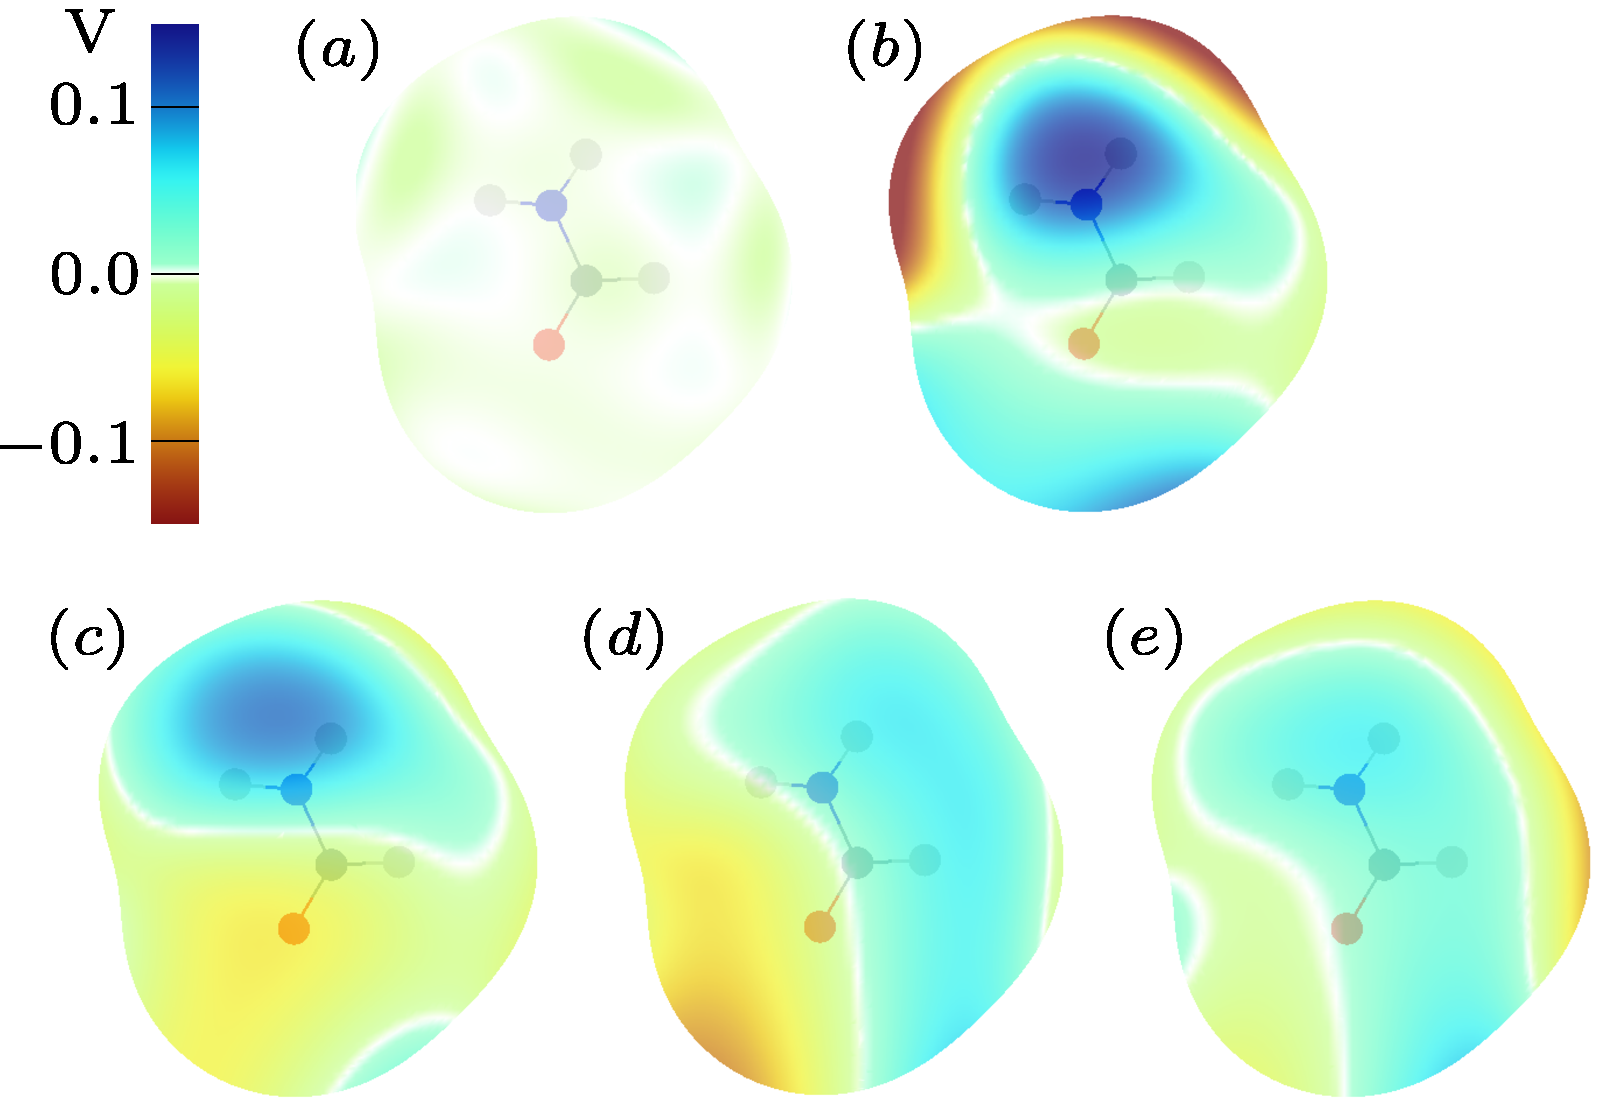
\includegraphics[scale=0.5,viewport=200 0 600 500]{pictures/point-charge-models.pdf}
\end{center}
\caption{Errors in potentials due to point-charge and
  distributed-multipole models for the 
electrostatic potential of formamide on a surface at 1.8 van der Waals
radii. The maps show the difference between the exact potentials
calculated from an aug-cc-pVQZ wavefunction and $(a)$ rank~5 DMA $(b)$
DMA charges only, $(c)$ charges fitted to DMA rank 5 using {\sc
  Mulfit}, $(d)$ charge of iterated stockholder atoms (ISA), $(e)$
CHELPG potential-derived charges. For an interacting charge of $0.5e$,
$0.1\,$V corresponds to about 5\kJpermol.}
\label{fig:formamide}
\end{figure}

\emph{If you need a point-charge model, do not use the atom charges from
GDMA.} The effects of atomic distortions caused by chemical bonding are
described in GDMA by the dipoles and higher moments, and simply
omitting those will give very poor results. For good results you need
to include dipoles and quadrupoles at least. However, some
applications can only handle point charge models, so it is sometimes
necessary to provide them. There are several possibilities,
illustrated in Fig.~\ref{fig:formamide}, which shows the difference
between the electrostatic potential of each of several models and the
exact potential evaluated as the interaction energy of a unit charge
with the electron density. The electron density and all models were
evaluated using the aug-cc-pVQZ basis, and the potential maps
were prepared using the {\sc Orient} program\cite{Orient4.8}.
Fig.~\ref{fig:formamide}(a)
shows the difference for the DMA to rank 5, for which the RMS error is
0.0026V. Fig.~\ref{fig:formamide}(b) shows the potential due to the
point charges of the DMA model only. This is clearly unsatisfactory,
with an r.m.s error of 0.07V and a maximum error of nearly 0.2V. 
One recommended procedure is 
to use the {\sc Mulfit} program of \citeauthor{WinnFR97}
\cite{WinnFR97,FerenczyWR97}, which approximates the atomic dipoles and higher 
moments by means of charges on neighbouring atoms. ({\sc Mulfit} can also be used
to refine a more detailed description, for example with multipoles up
to quadrupole, by approximating the contributions of the octopoles and
hexadecapoles.) Fig.~\ref{fig:formamide}(c) illustrates the improvement
that can be obtained in this way; the r.m.s. error is 0.041V. 
Fig.~\ref{fig:formamide}(d) was obtained using the charges from an
iterated stockholder atom (ISA) description\cite{MisquittaSF14}, calculated
using the {\sc CamCASP} program of Misquitta \& Stone\cite{CamCASP5.9},
and Fig.~\ref{fig:formamide}(e) was obtained using CHELPG charges,
calculated using Gaussian03. The r.m.s. differences for these cases
are 0.044V and 0.034V respectively. Note that the ISA method yields a
complete distributed-multipole description, not just the charge model
used here.

The {\sc Mulfit} package is included with the GDMA distribution, by
permission of its authors. See the instructions included with that
package for details of its use.

\section{Example data files}

A number of examples are provided in the \verb/examples/ directory and
its subdirectories, together with output files. The script
\verb/run.tests/ in the \verb/examples/ directory runs these
calculations automatically and compares the results with the output
files provided. 

\section{Program limits}

In version 2.2.02 and later, the arrays used by the program are allocated as
required, so there should be no problems with large molecules or large
basis sets. The maximum number of sites is arbitrarily set at 16 more
than the number of atoms, and this should be sufficient, but if more
sites are needed it will be necessary to increase the value of
\texttt{nextra} near the top of the gdma.f90 file and recompile.


\section{Citation}

Please use the citation as in Ref.~\citenum{Stone05b} when referring
to the program.


\section{Revision notes}

\textbf{Version 2.3.0} allows for basis sets that include $h$
functions. Both Gaussian and Psi4 can produce the necessary fchk
files. An unnecessary limit of 16 on contraction depth has been
removed.

\textbf{Version 2.2.02} uses dynamic allocation of arrays, so that
there are no arbitrary limits on the size of the molecule or the basis
set. There is an arbitrary limit on the number of sites, as noted
above, but it should be adequate for most if not all cases.

\textbf{Version 2.2} incorporates the minor but significant change
that the radius assigned by default to hydrogen atoms is half the default
radius for other atoms. Calculations involving H atoms with default
radii will give results that are different from earlier versions.

\textbf{Version 2.1} provides for printing multipole moments in SI
units as an alternative to the standard atomic units.

\textbf{Version 2.0} This version of the program can handle basis
functions up to $g$. It also provides for real-space apportionment
of the charge density arising from low-exponent primitives, instead
of the allocation of all multipoles from a particular
primitive-function overlap density to the nearest site.

\textbf{Version 1.3} Explicit type declarations introduced. This dealt
with an apparent bug in the Portland compiler, which gave wrong
results when implicit declarations were used.

\textbf{Version 1.2} Modified to handle new features in the Gaussian03
formatted fchk files.

\pagebreak
\bibliography{macros,all}

\end{document}
